\chapter{Background}

\lettrine{A}{n} in-depth discussion of the background associated with the project is presented, discussing specific topics driving the approach taken to solving the problem. The literature review is divided into four sections:
\begin{enumerate}
  \item Spacecraft trajectory guidance at large, for which solar sail guidance is a subset;
  \item Feedback guidance laws, particularly the \textit{Q-Law} derived from Lyapunov control theory;
  \item Special considerations needed for solar sails beyond conventional low-thrust spacecraft;
  \item Approaches to solar sail guidance, particularly planetocentric orbital maneuvering.
\end{enumerate}

\section{Spacecraft Trajectory Guidance at Large}

This section covers essential aspects of spacecraft orbits, followed by a discussion of various approaches used to develop guidance laws for orbital maneuvering. Techniques for low-thrust spacecraft are given focus, as those are most relevant to solar sails.

\subsection{The Planetocentric Guidance Problem}
The general problem of planetocentric orbital maneuvering refers to altering the orbit of a spacecraft around a parent celestial body from some initial orbit to a final target orbit. (Note that this is different from \textit{rendezvous}, which adds a further constraint that the spacecraft must reach a certain point along the target orbit at a specific time, i.e. to meet with a spacecraft already in that target orbit.)

\begin{figure}[H]
\tdplotsetmaincoords{30}{30}
\begin{tikzpicture}[tdplot_main_coords,scale=1]
    \coordinate (O) at (0, 0, 0);
    \coordinate (SC) at ({9/sqrt(2)}, {9/sqrt(2)}, 0);
    % Orbit 1
    \begin{scope}[plane x={({1/sqrt(2)}, {1/sqrt(2)}, 0)}, plane y={(-0.5, 0.5, {1/sqrt(2)})}, canvas is plane]
    % Grid
    \begin{scope}[densely dotted, green!50!black]
    \draw (-1, 0, 0) -- (9, 0, 0);
    \draw (0, -1.8, 0) -- (0, 1.8, 0);
    \end{scope}
    \draw[green!50!black, thick, fill=green!50!black, fill opacity=0.2] (4, 0, 0) ellipse (5cm and 3cm);
    \draw (9, -0.5) node[below right, green!50!black, text width=4cm]{Initial Orbit};
    \end{scope}
    % Orbit 2
    \begin{scope}[plane x={(1, 0, 0)}, plane y={(0, 1, 0)}, canvas is plane]
    % Grid
    \begin{scope}[densely dotted, red!50!black]
    \draw (-2, 0, 0) -- (8, 0, 0);
    \draw (0, -3, 0) -- (0, 3, 0);
    \end{scope}
    \draw[red!50!black, thick, fill=red!50!black, fill opacity=0.2] (3, 0, 0) ellipse (5cm and 4cm);
    \draw (8, 0) coordinate (PP) node[below right, red!50!black, text width=5cm]{Target Orbit};
    \end{scope}
    % SC
    \fill[black] (SC) circle(0.1cm);
    \draw (SC) node[right]{Spacecraft};
    % Earth
    \fill[earthblue] (0, 0) circle(0.5cm);
    % Axes
    \begin{scope}[-latex, thick]
        \draw (O) -- ++ (2,0,0);
        \draw (O) -- ++ (0,2,0);
        \draw (O) -- ++ (0,0,2);
    \end{scope}
    % Arrow
    \coordinate (AA) at ($(SC)!0.25!(PP)$);
    \coordinate (BB) at ($(SC)!0.9!(PP)$);
    \draw[densely dashdotted, thick, -latex] ($(O)!1.2!(AA)$) to[bend left = 20] ($(O)!1.2!(BB)$);
\end{tikzpicture}
\caption{Cartoon illustration of the planetocentric orbital maneuvering guidance problem.}
\label{fig:guidance_problem}
\end{figure}

Solving the guidance problem refers to generating a sequence of applied thrust vectors which modify the spacecraft's orbit accordingly. Since the solution is generally not unique, the space of all valid guidance solutions can be searched for those which result in the shortest time of flight or the least propellant expenditure, for example. Hence, the guidance problem is often considered approached as an optimization problem \cite{yam2011low}.

\subsection{Description and Evolution of Spacecraft Orbits}

Orbits (in the context of the two-body problem) are described using a set of 6 orbital elements \cite{book:1487513}. Keplerian orbital elements are the most prolific, but there exist alternative formulations of two-body spacecraft orbits which also result in 5 elements specifying orbital geometry/orientation and 1 element representing time.

Some examples:
\begin{itemize}
  \item Keplerian Elements \(\{a, e, i, \Omega, \omega, \theta\}\)
  \item Modified Equinoctial Elements \(\{p, f, g, h, k, L\}\) \cite{walker1985set}
  \item Gooding Universal Elements  \(\{\alpha, q, i, \Omega, \omega, \tau\}\) \cite{gooding_universal_elements}
\end{itemize}

Altering the orbit of a spacecraft to solve the guidance problem involves changing its orbital elements. The process of solving for the evolution of orbital elements in time is known as \textit{orbit propagation}.

Cowell's method \cite{book:1487513} is a well-known way of propagating general spacecraft trajectories in Cartesian state space. Typically this involves integrating equations of motion derived from Newton's second law in a form similar to the following:

\begin{equation}
  \diff[2]{}{t}{\boldsymbol{r}} = -\frac{\mu}{||\boldsymbol{r}||^3} \boldsymbol{r} + \boldsymbol{f}_\mathrm{p} \label{eq:cowells_method}
\end{equation}
Wherein \(\boldsymbol{f}_\mathrm{p}\) is some perturbing acceleration (i.e. unrelated to point-mass gravity of the central body) and \(\boldsymbol{r}\) is the position vector of the spacecraft (both expressed in an inertial frame). Although simple at first glance, a difficulty of working in Cartesian coordinates for spacecraft guidance is that all six values of the state vector (position and velocity) change in time, regardless of the presence of perturbations. Additionally, describing the geometry of an orbit in terms of Cartesian state is not as straightforward as using orbital elements.

\textbf{Variational Methods for Orbit Propagation}

Variational equations of motion are ordinary differential equations giving the time derivatives of orbital elements when subject to a perturbing acceleration, such as thrust from a propulsion system. Taking Keplerian elements as an example, they take the form:
\begin{equation*}
  \diff{}{t}
  \begin{bmatrix}
    a \\e\\i\\ \Omega \\ \omega \\ \theta
  \end{bmatrix}
  = A \boldsymbol{f}_\mathrm{p} + \boldsymbol{b}
\end{equation*}
Where \(A \in \mathbb{R}^{6\times6}\), \(\boldsymbol{b} \in  \mathbb{R}^{6}\), and typically only the last entry of \(\boldsymbol{b}\) is nonzero (i.e. the other 5 orbital elements are invariant when there is zero perturbing acceleration).

When posed in terms of variational equations of motion, the guidance problem becomes one of determining the perturbing acceleration needed at each instant in time to \textbf{change the orbital elements of the spacecraft which describe the geometry and orientation of the orbit} (e.g. in the case of Keplerian elements, \(a, e, i , \Omega, \omega\)).

Compared to Cowell's method, working directly in orbital elements dramatically simplifies the analysis of guidance laws, particularly in discussing convergence to the target orbit.

\textbf{Comparison with Classical Orbital Maneuvering Theory}

Classical orbital maneuvering theory employs brief, high-thrust maneuvers which are approximated as impulses, leading to a sequence of discrete orbits constituting a maneuver, and removing the need to analyze trajectories in terms of continuous equations of motion. Impulse-based maneuvering theory has been extensively studied and is commonly taught at the undergraduate level, as demonstrated by books such as Ref. \cite{book:1487513}. On the other hand, low-thrust guidance requires time integration of differential equations, making the majority of analysis \textbf{heavily-reliant on numerical simulation}. One common approach used for solving the guidance problem for a (low-thrust) solar sail spacecraft is to \textbf{integrate the variational equations of motion}.

\subsection{The Case for Modified Equinoctial Elements}
The 5 Keplerian elements describing the geometry and orientation of an orbit are the semi-major axis (\(a\)), eccentricity (\(e\)), inclination (\(i\)), right ascension of the ascending node (\(\Omega\)), and argument of periapsis (\(\omega\)). The remaining orbital element used to represent time is the true anomaly (\(\theta\)). A significant challenge associated with using Keplerian elements and their respective variational equations in trajectory analysis are the \textbf{singularities} which occur for many types of orbits (e.g. circular orbits, zero-inclination orbits). Although no orbits are perfectly circular or zero-inclination in practice, the singularities appearing in both the orbital elements themselves and their associated variational equations cause numerical issues in simulations.

Common solutions to this include adding ``deadbands'' to the values of eccentricity and inclination, such when they are decremented under some threshold (e.g. \(|e| < 10^{-4}\)), their value is clamped to the lower bound until their rates of change become positive. This is the approach taken by Petropoulos (2004) \cite{petropoulos2004low} to avoid reaching singularities.

Modified equinoctial orbital elements defined by Walker et. al (1985) \cite{walker1985set} remove singularities in all cases except for a perfectly retrograde equatorial orbit, and present many numerical conveniences for analysis. They are defined from Keplerian elements as follows:
\begin{align*}
  p & = a \left(1-e^2\right)    & h & = \tan(i/2) \cos \Omega    \\
  f & = e \cos(\omega + \Omega) & k & = \tan(i/2) \sin \Omega    \\
  g & = e \sin(\omega + \Omega) & L & = \Omega + \omega + \theta
\end{align*}
In contrast to Keplerian elements, the modified equinoctial elements (\(f, g, h, k\)) describing the orientation of the orbit represent ratios instead of angles, and are order unity (when \(i \in [-\ang{90}\, \ang{90}]\)). Perfectly circular and equatorial orbits are handled without issues in the variational equations of motion (shown later in Equation \ref{eq:equinoctial_eom_3d}).

The heavy dependence of numerical simulation for the analysis low-thrust spacecraft trajectories makes modified equinoctial elements a good basis for developing a guidance law.

\subsection{Global Optimization Methods for Low-Thrust Trajectories}

One common approach used for low-thrust trajectory planning is posing the guidance problem as a global optimization problem. At a high level, there exist two main classes of methods: direct and indirect methods, along with variants thereof. These are presented in depth in a survey of the state of the art by Morante et al. (2021) \cite{morante2021survey}, but the essential points are discussed here. Note that global methods often employ a Cartesian state formulation instead of orbital elements.

Both methods construct a sequence (i.e. a time history) of control inputs which bring the spacecraft to a targeted state. Both methods also discretize the problem by assuming a certain form for the control inputs (e.g. piecewise polynomials). Direct methods solve for unknown coefficients using pseudospectral or other collocation-based methods through integration of the equations of motion and direct evaluation of the functional to be optimized. Indirect methods (also referred to as adjoint, co-state, or primer vector methods) use variational techniques and Lagrangian multipliers to produce systems of equations with sufficient constraints for optimality which are then solved to get the unknown coefficients. As described by Kelly (2015) in an introductory overview paper of global optimization \cite{kelly2015transcription}, direct methods find coefficients to minimize a functional, while indirect methods solve a system of equations which ``set the gradient of the functional to be zero''.

For interplanetary missions, the timescale of the astrodynamics (i.e. the period of orbits around the Sun) is similar to the timescale of the optimization problem (i.e. the time of flight), making the problem computationally tractable through use of a coarse discretization. The Sims-Flanagan method, a direct method, is highly amenable for interplanetary trajectories \cite{sims1997preliminary, yam2011low}. Collocation-based methods (e.g. Gauss pseudospectral methods) are used in similar applications \cite{fahroo2002direct, narayanaswamy2020comparison}.

A critical weakness of global optimization approaches for trajectory planning is their dependence on an initial guess. Indirect methods in particular struggle with stably converging to a solution when presented with a poor initial guess. For simple interplanetary trajectories, intuition is sufficient to kickstart an optimization, but the complex nature of orbital transfers around a planet is considerably less intuitive.

As discussed in the introduction, a challenging aspect of planetocentric orbital maneuvering is the mismatch in timescales between orbital periods and time of flight. Referred to as \textbf{multi-revolution transfers}, trajectories making a large number of revolutions around a planet require basis functions with sufficiently high spatial frequency to accurately capture the ``curvature'' of the orbits. An extremely low-thrust propulsion system such as a solar sail may need hundreds of revolutions to raise its orbit, requiring either a very high order basis or a large number of basis functions -- both of which result in a challenging computational workload.

Consequently, this project focuses on an entirely different approach to spacecraft guidance -- locally optimal feedback guidance.

\section{Feedback Guidance Laws}
Classical control theory is built upon the idea of simple feedback control loops. Although designed without any guarantees for global optimality, they are simple to implement, and can be tuned to get near-optimal performance.

The same idea has been applied to guidance in two main forms: thrust-blending and Lyapunov control. Both approaches use formulations using orbital elements for state representation. In both cases, the key idea is to take the difference between the current value and target value for each orbital element, and produce a control input which decreases the error at each timestep. Removing the dependence of modelling a coupled global trajectory dramatically decreases computational complexity, and has the added benefit of being easy to run ``online'' with simulators in a feedback loop.

Thrust-blending (also referred to as blended control) methods find control inputs which independently maximize the rate of decrease of the error for each of the orbital elements, and take a linear combination of the individual inputs. This is examined more thoroughly in the survey by Morante et al. (2021) \cite{morante2021survey}.

Lyapunov methods can be thought of as a variant of thrust-blending methods, by using a heuristic to weigh the decrease in error for each orbital element by an optimality criterion. The specific linear combination taken is the one which maximizes the rate of decrease of some scalar function, described in the next section.

\subsection{Lyapunov Methods}
A brief primer on Lyapunov control theory is presented, based on an explanation from the fundamental paper of planetocentric Lyapunov-based guidance by Ilgen (1994) \cite{ilgen1994low}.

Consider a dynamic system with state \(x(t) \in \mathbb{R}^n\) a control input \(u \in \mathbb{R}^m\) governed by some differential equation \(f : \mathbb{R}^n \times \mathbb{R}^m \to \mathbb{R}^n\) s.t. \(\dot{x}(t) = f(x(t), u)\).

Consider a function \(V: \mathbb{R}^n \to \mathbb{R}\), called a \textbf{potential function or control-Lyapunov function}, which maps each state value to some scalar. Intuitively, this can be thought of as analogous to the potential energy of the system, which vanishes at some point \(x = \hat{x}\), e.g. a mass attached to a spring, wherein \(V(x) = \frac{1}{2}(x-\hat{x})^2\)

This dynamic system is said to be \textbf{Lyapunov stable} iff a potential function can be found which meets the following conditions:
\begin{enumerate}
  \item \(V(x) > 0\  \forall \ x \neq \hat{x}\)
  \item \(V(\hat{x}) = 0\)
  \item There exists some \(u\) for all \(x \in \mathbb{R}^n\) s.t.
        \begin{align*}
          \dot{V}= \nabla V(x) \cdot \dot{x}(t) & = \nabla V(x) \cdot f(x, u) < 0
        \end{align*}
        where \(\nabla V(x)\) means \(\diff{V}{{x_i}} = \left\{\diff{V}{{x_1}}, ..., \diff{V}{{x_n}}  \right\}\)
\end{enumerate}
Or in other words:
\begin{itemize}
  \item \(V(x)\) is positive definite
  \item For every state, there exists a control input which decreases \(V(x)\) in time.
\end{itemize}

Over time, this is guaranteed to drive the state towards \(x = \hat{x}\), so long as the stabilizing control input is provided.

This is a powerful idea, because it can be used both as a means to prove the stability of a system, and also as a means of developing a feedback control law \(u = u(x, t)\)

Solving for the value of \(u\) at each value of \(x\) such that \(\dot{V}\) is minimized produces a \textbf{locally optimal feedback control law}.

By introducing an optimality criterion, a unique solution can be obtained at each timestep. Lyapunov control is hence a natural extension of thrust blending.

\subsection{Early Control-Lyapunov Functions}

Ilgen's paper proposes a potential function which is a linear combination of the square of the difference between each orbital element and its target value. Formulated in Keplerian elements, it is given as:
\begin{equation}
  V = \frac{1}{2} \left[P_1 \frac{(a - \hat{a})^2}{R_e^2} + P_2 (e - \hat{e})^2 + P_3 (i - \hat{i})^2 + P_4 (\Omega - \hat{\Omega}) + P_5 (\omega - \hat{\omega})^2  \right]
  \label{eq:ilgen_potential}
\end{equation}
where hatted values refer to target orbital elements, and \(P_i, i \in \{1, ..., 5\}\) are weighting factors.

At each timestep, the only thing needed to compute the control input is the current state of the spacecraft -- there is \textbf{no dependence on past or future states}, making the guidance law extremely cheap computationally.

Additionally, given the relatively simple nature of the potential function, it is possible to derive analytical expressions for the control input. However, given that Ilgen's potential function is expressed in Keplerian elements, there are singularities in the derivatives of \(V\).

Nonetheless, Ilgen demonstrates \textbf{nearly time-optimal behaviour} from this guidance law, making it a competitive alternative to global methods.

Importantly, Ilgen demonstrates guaranteed convergence to the final target orbit under certain limiting conditions. This is remarkable, as \textbf{no knowledge of the global solution is needed} to converge to the target orbit. However, a complete analysis of convergence in the general case is not given.

This paper highlights many of the key strengths and weaknesses of Lyapunov methods for guidance. While Lyapunov methods are simple to implement, cheap to simulate, and performant, it is challenging to rigorously analyze the performance of feedback guidance laws, particularly with regards to convergence guarantees and convergence rate. The lack of coupling to the global solution makes it difficult to robustly ascertain that a locally optimal solution can be extended to the global domain.

Another example of a control-Lyapunov guidance law is demonstrated by Naasz \cite{naasz2002classical}.

A notable contemporary development in Lyapunov-based planetocentric orbit maneuvering guidance is a family of guidance laws spawned from the \textit{Q-Law}.

\subsection{The \textit{Q-Law} Family}
The \textit{Q-Law} was developed by Petropoulos \cite{petropoulos2004low} using a potential function of the form:
\begin{equation}
  Q = (1 + W_P P) \sum_{\moe} W_\moe S_\moe \left(\frac{\moe - \hat{\moe}}{\dot{\moe}_{\max}} \right)^2, \ \  \moe \in \{a, e, i, \Omega, \omega\}
  \label{eq:q_law_petropulos}
\end{equation}
where \(P\) is a penalty function used to impose constraints, \(S_\moe\) is a scaling function for each orbital element, and \(W_\sigma, \sigma \in \{P, a, e, i, \Omega, \omega\}\) are weights. \(\hat{\moe}\) represents target orbital elements, and \(\dot{\moe}_{\max}\) represents the maximum attainable rate of change in each orbital element across the course of an orbit (i.e. across all values of \(\theta\)) and across all thrust directions (assuming a propulsion system with fixed thrust).

\(Q\) is described as a ``proximity quotient''; each term in the summation can be thought of as the square of the minimum time needed to drive the error in a single orbital element to zero.

One of the key brilliancies of the approach is implementing a means to compensate for \textbf{how ``easy'' it is to change a given orbital element} (through \(\dot{\moe}_{\max}\)). Orbital elements which have a lower possible maximum rate of change are weighed with more importance by the potential function. This mechanism allows for the error in each orbital element to ``balance out'' over time, which is important for practically ensuring stability and convergence.

Weighing \(Q\) by \(\dot{\moe}_{\max}\) informs the application of \textbf{control effort} such that the ``most difficult'' orbital elements are addressed first, and ensures that no orbital element gets left behind.

\(\dot{\moe}_{\max}\) can be computed from the variational equations of motion, and results in an analytical expression for the derivatives of \(Q\). Note that when formulated in modified equinoctial elements, analytical approximations are used for \(\dot{\moe}_{\max}\) \cite{vargaperez2016, sanjeev2023}.

Petropoulos' original paper has been built upon numerous times for different applications, including rendezvous \cite{sanjeev2023}. Varga and Pérez (2016) \cite{vargaperez2016} give an implementation in modified equinoctial elements, along with a study on optimizing the values of \(W_\sigma, \sigma \in \{P, a, e, i, \Omega, \omega\}\). Proceeding work on the Q-Law has adopted the modified equinoctial element formulation \cite{sanjeev2023} for its better performance.

The \textit{Q-Law} family has demonstrated remarkably good performance when tested in higher fidelity studies, incorporating eclipse effects (i.e. rendering electric propulsion inoperable when occluded from sunlight), and J2 perturbation \cite{vargaperez2016}. Although solar sails are a relatively fresh application for this type of guidance law, the long history of good performance under challenging conditions makes it a good foundation to build upon for this project.

\section{Considerations for Solar Sails}
Solar sails are a propulsion method requiring no propellant expenditure to produce thrust. The principle of operation is based on conservation of momentum in the reflection of incident photons from the Sun. Challenges associated with performing controlled maneuvers using solar sails are described, with discussions of implications on spacecraft guidance. Fundamental principles are taken with reference to McInnes (1999) \cite{mcinnes}.

The most challenging aspects of bringing solar sails into reality are not actually related to trajectory planning; truthfully, the greatest issues lie in the manufacturing and production of solar sails; material science and mechanical design remain the greatest barriers to the widespread adoption of solar sails \cite{mcinnes}. On top of that, attitude control is a fundamental precursor to thrust control, and is still in a highly developmental stage \cite{choi2015structural}.

With that said, guidance is still an important and challenging problem for solar sailing. An important fact to consider is that real solar sails behave very differently from an ideal flat sail. As discussed by Polyakhova (2018) in a review of solar sailing missions, models describing the thrust produced by solar sails continue to change with every new spacecraft built and flown \cite{polyakhova2018solar}.

In a perfectly idealized model, thrust is produced exactly in the direction of the sail normal, and the cone angle can be as great as \ang{90}. Real solar sails have limits on maximum allowable cone angle due to considerations for attitude control or because the reflective material of the sail behaves non-ideally at shallow incidence angles (e.g. absorption and re-radiation effects). Due to these same reflectivity effects, the resultant thrust vector is not always aligned perfectly with the sail normal. This is illustrated in Figure \ref{fig:sail_reflectivity_comparison} below.

\begin{figure}[H]
  \centering
  \begin{subfigure}[t]{0.49\textwidth}
    \centering
    \begin{tikzpicture}[scale=0.98]
      \coordinate (O) at (0, 0);
      \coordinate (Sun) at (190:4cm);
      \coordinate (T) at (220:1cm);
      \begin{scope}[black!50]
        \draw[ultra thick] (O) ++ (130:2cm) -- ++(-50:4cm);
        \draw (O) ++(220:0.1cm) ++ (130:2cm) -- ++(-50:4cm);
      \end{scope}
      \draw[-latex, dashed, purple!70!black] (O)  ++(220:2cm) -- ++(40:4cm) node[above]{Sail Normal (\(\hat{n}\))};
      \draw[-latex, color=orange!70!black, thick] (O) -- ++(40:1.5cm) node[right]{\footnotesize{Thrust (\(\vec{F}\))}};
      \begin{scope}[cyan!50!black]
        \draw[-latex, thick] (Sun) -- (O) node[midway, above=4pt] {\footnotesize{Incident Light \(\hat{u_i}\)}};
        % Reflected rays
        \draw[-latex] (O) -- ++(-100:2.5cm) node[right]{\footnotesize{Reflected Light}};
      \end{scope}
      % Draw Sun
      \fill[color=yellow] (Sun) circle(0.5cm);
      % angles
      \draw pic["\footnotesize{\(\varphi\)}", draw=black, text=black, |->, angle eccentricity=1.4, angle radius=1.3cm] {angle=Sun--O--T};
    \end{tikzpicture}
    \caption{Perfectly reflecting sail.}
    \label{fig:perfect_sail}
  \end{subfigure}
  \begin{subfigure}[t]{0.49\textwidth}
    \centering
    \begin{tikzpicture}[scale=0.98]
      \coordinate (O) at (0, 0);
      \coordinate (Sun) at (190:4cm);
      \coordinate (T) at (220:1cm);
      \begin{scope}[black!50]
        \draw[ultra thick] (O) ++ (130:2cm) -- ++(-50:4cm);
        \draw (O) ++(220:0.1cm) ++ (130:2cm) -- ++(-50:4cm);
      \end{scope}
      \draw[-latex, color=orange!70!black, thick] (O) -- ++(30:1cm) node[right]{\footnotesize{Thrust (\(\vec{F}\))}};
      \draw[-latex, dashed, purple!70!black] (O)  ++(220:2cm) -- ++(40:4cm) node[above]{Sail Normal (\(\hat{n}\))};
      \begin{scope}[cyan!50!black]
        \draw[-latex, thick] (Sun) -- (O) node[midway, above=4pt] {\footnotesize{Incident Light \(\hat{u_i}\)}};
        % Reflected rays
        \draw[-latex] (O) -- ++(-70:2cm) node[right]{\footnotesize{Reflected Light}};
        \draw[-latex] (O) -- ++(-80:2cm);
        \draw[-latex] (O) -- ++(-90:2cm);
      \end{scope}
      % Draw Sun
      \fill[color=yellow] (Sun) circle(0.5cm);
      % angles
      \draw pic["\footnotesize{\(\varphi\)}", draw=black, text=black, |->, angle eccentricity=1.4, angle radius=1.3cm] {angle=Sun--O--T};
    \end{tikzpicture}
    \caption{Real sail.}
    \label{fig:general_sail}
  \end{subfigure}
  \caption{Effects of non-ideal effects on solar sail thrust production.}
  \label{fig:sail_reflectivity_comparison}
\end{figure}

\subsection{Inherent Challenges of Dynamics}
Even in the case of a flat perfectly reflecting sail, there are two key obstacles complicating the application of low-thrust guidance theory to solar sail spacecraft.
\begin{enumerate}
  \item \textbf{Direction-Dependent Availability of Thrust}: The thrust produced by a solar sail is related to the cone angle \(\varphi\) by a factor of roughly \(\cos^2(\varphi)\) (see Equation 2.22 of Ref. \cite{mcinnes}). Thrust falls off considerably as the sail becomes misaligned with the direction of incident light, and drops to zero for \(|\varphi| > \ang{90}\). This means that at any instant in time, only a single hemisphere of thrust directions can be realized, with the orientation of the hemisphere being dependent on the position of the Sun -- a quantity which cannot be directly controlled. This is illustrated in Figure \ref{fig:thrust_availability}.
  \item \textbf{Time/Position-Dependent Availability of Thrust}: The availability of thrust depends on a clear line of sight to the Sun. In eclipse, no light hits the sail, and no thrust is produced. This is illustrated in Figure \ref{fig:eclipse}. For spacecraft in low orbits above a planet, the time spent in eclipse represents a substantial fraction of the orbital period. More importantly, for a planetocentric orbit, the position of the parent planet around the Sun directly affects the direction of incident sunlight hitting the spacecraft and hence directional thrust availability. This is revisited in Section \ref{sec:solar_sail_guidance}.
\end{enumerate}
\begin{figure}[H]
  \centering
  \begin{subfigure}[t]{0.49\textwidth}
    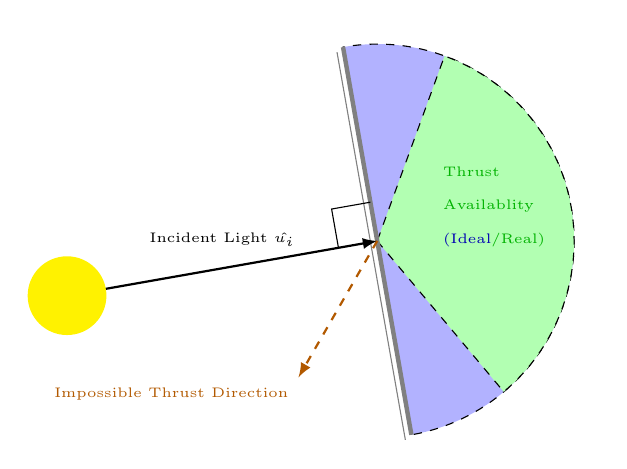
\begin{tikzpicture}
      \coordinate (O) at (0, 0);
      \coordinate (Sun) at (190:4cm);
      \coordinate (T) at (220:1cm);
      \filldraw[dashed, fill=blue!30!white] (O) -- ++(-80:2.5cm) arc(-80:100:2.5cm) -- cycle;
      \filldraw[dashed, fill=green!30!white] (O) -- ++(-50:2.5cm) arc(-50:70:2.5cm) node[midway, left=0cm, text width=1.5cm, text=green!70!black]{\tiny{Thrust \newline Availablity\newline \textcolor{blue!70!black}{(Ideal}/Real)}}-- cycle;
      \begin{scope}[black!50!white]
        \draw[ultra thick] (O) ++(-80:2.5cm) -- ++(-80:-5cm);
        \draw (O) ++(220:0.1cm) ++(-80:2.5cm) -- ++(-80:-5cm);
      \end{scope}
      \draw (O) ++(190:0.5cm) -- ++(100:0.5cm) -- ++(10:0.5cm);
      \draw[-latex, thick] (Sun) -- (O) node[midway, above=4pt] {\tiny{Incident Light \(\hat{u_i}\)}};
      \draw[-latex, thick, dashed, orange!70!black] (O) -- +(-120:2cm) node[below left, text=orange!70!black]{\tiny{Impossible Thrust Direction}};
      % Draw Sun
      \fill[color=yellow] (Sun) circle(0.5cm);
    \end{tikzpicture}
    \caption{The direction of produced thrust is limited for solar sails.}
    \label{fig:thrust_availability}
  \end{subfigure}
  \begin{subfigure}[t]{0.49\textwidth}
    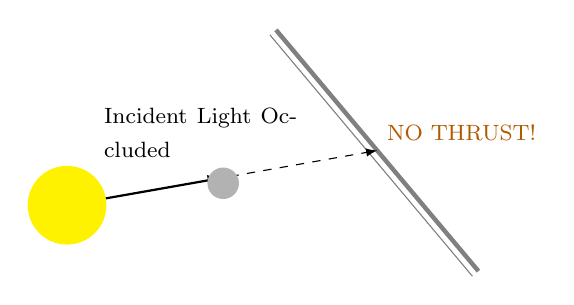
\begin{tikzpicture}
      \coordinate (O) at (0, 0);
      \coordinate (Sun) at (190:4cm);
      \coordinate (E) at (192:2cm);
      \coordinate (T) at (220:1cm);
      \begin{scope}[black!50!white]
        \draw[ultra thick] (O) ++ (130:2cm) -- ++(-50:4cm);
        \draw (O) ++(220:0.1cm) ++ (130:2cm) -- ++(-50:4cm);
      \end{scope}
      \draw (O) node[above right, text=orange!70!black]{\footnotesize NO THRUST!};
      \draw[-latex, thick] (Sun) -- ++(10:2cm);
      \draw[-latex, dashed] (Sun) -- (O) node[midway, above=4pt, text width=3cm] {\footnotesize{Incident Light Occluded}};
      % Draw Sun and Earth
      \fill[color=yellow] (Sun) circle(0.5cm);
      \fill[color=black!30] (E) circle(0.2cm);
    \end{tikzpicture}
    \caption{Solar sails produce no thrust in eclipse.}
    \label{fig:eclipse}
  \end{subfigure}
  \caption{Key challenges associated with solar sail thrust.}
  \label{fig:sail_challenges}
\end{figure}
Both of these effects are present to a lesser degree in spacecraft using electric propulsion; solar arrays require Sun exposure, but are typically made to rotate so that they can track the Sun independently of the direction of the engines. Solar sails pose a more extreme set of challenges for maneuvering, stemming from their principle of operation.

\subsection{Diversity of Sail Geometries and Materials}
McInnes (1999) \cite{mcinnes} discusses several different solar sail geometries and reflectivity models with considerably different forms.

Real solar sails do not adhere to perfectly flat geometries due to deformation effects \cite{sakamoto2006effect}, and can even be designed intentionally with non-flat geometry for enhanced attitude control capabilities \cite{felicetti2016attitude}.

IKAROS (2010) featured variable-reflectivity materials on its surface for attitude control \cite{tsuda2013achievement}, and sail materials are an ongoing field of development, as discussed in a review of the state of the art by NASA (2011) \cite{johnson2011status}.

The key point to be made is that fixating upon a certain dynamic model for solar sails is overly restrictive for adequate consideration of future solar sail designs.

Note that there is work done by Rios-Reyes et al. (2005) \cite{rios2005generalized} and Tsunda et al. (2013) \cite{tsuda2013generalized} on generalizing solar sail dynamics models. These models allow for arbitrary geometries and surface reflectivity properties, but have a large number of parameters. For the sake of simplicity, integrating such a model into the guidance law for this project is not considered.

\subsection{Attitude Dynamics}
Solar sail spacecraft have limited attitude agility; as a first approximation, angular rates of about \(\ang{15}\) per hour are achievable \cite{choi2015structural}. Even with this crude notion of maneuverability, maneuvers in orbits where the orbital period is shorter than a few hours (such as LEO) become difficult with solar sail spacecraft. Such considerations should be made when making a guidance law, so that the time history of commanded thrust directions can be realized by the attitude controller.

Incorporating attitude constraints is complex; attitude control often depends on radiation pressure for maneuvering (e.g. tip vanes, LCD panels), and hence the maximum attainable attitude rates vary with the orientation of the spacecraft. Also, as previously mentioned, there are also limits imposed on the angles of the sail relative to the Sun, which continuously vary in time as the Sun moves.

Considering attitude dynamics in a globally optimal method is challenging, since the above constraints often cannot be expressed in a simple form. Even with feedback methods, directly incorporating such constraints into a guidance law dramatically increases its complexity. Therefore, the majority of approaches to solar sail guidance make simplifications to ignore certain aspects of attitude dynamics.


\section{Solar Sail Guidance}
\label{sec:solar_sail_guidance}
Traditional solar sail guidance has focused on heliocentric trajectories. Analytical analysis of inward and outward spiral trajectories around the Sun are discussed by McInnes (1999) \cite{mcinnes}. However, the focus of this literature review is on planetocentric orbital maneuvering.

In planetocentric orbits, the issues of directional thrust availability and eclipse are more severe than when around the Sun. For instance, the ``hemisphere'' of allowable thrust directions (see Figure \ref{fig:thrust_availability}) makes a full revolution during each orbit around the Sun, and therefore a solar sail in heliocentric orbit can apply thrust in nearly all directions over the course of a single orbit. On the other hand, the position of the Sun relative to a spacecraft barely changes over the course of a single orbit around a planet, which greatly restricts the possible space of thrust directions. Consider Figure \ref{fig:angle_availability} for an illustration of this. Furthermore, as already mentioned, eclipse is a common occurrence in low orbit around a planet, while it is effectively nonexistent when orbiting the Sun.

\begin{figure}[H]
  \centering
  \begin{subfigure}[t]{0.45\textwidth}
    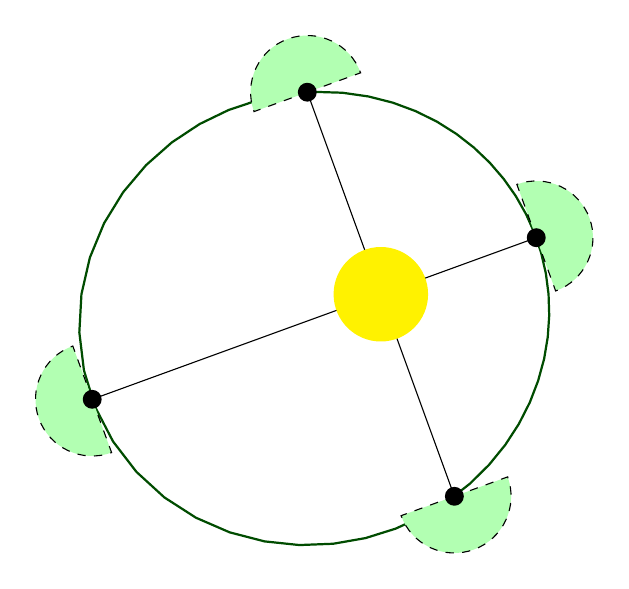
\begin{tikzpicture}[scale=1.2]

    \coordinate (S) at (0, 0);

    \pgfmathsetmacro{\e}{0.3} % set = keep float
    \pgfmathsetmacro{\p}{2.5}
    \pgfmathsetmacro{\aop}{20}

    % Orbits
    \foreach \s in {1,...,50}
        {
            \pgfmathsetmacro{\theta}{360/50*(\s-1)}  % define angle
            \draw (S) +(\theta:{\p*(1-\e^2)/(1 + \e*cos(\theta-\aop))}) coordinate (ORB1\s);
        }
    \draw[green!30!black, thick] (ORB11) foreach \s in {2,...,50}{-- (ORB1\s)} -- cycle;

    \pgfmathsetmacro{\arcsize}{0.6}

    \foreach \theta in {20, 110, 200, 290}
        {
            \pgfmathsetmacro{\radius}{\p*(1-\e^2)/(1 + \e*cos(\theta-\aop))}
            \draw (S) -- ++(\theta:\radius) coordinate (SC\theta);
            \filldraw[dashed, fill=green!30!white] (SC\theta) -- ++(\theta+90:\arcsize) arc(\theta+90:\theta-90:\arcsize) -- cycle;
            \fill[black] (SC\theta) circle (0.1cm);
        }

    \fill[yellow] (S) circle (0.5cm);

\end{tikzpicture}
    \caption{Heliocentric trajectories: thrust availability depends only on the orientation of the spacecraft orbit relative to its parent body (the Sun).}
    \label{fig:angle_availability_sun}
  \end{subfigure}
  \hfill
  \begin{subfigure}[t]{0.45\textwidth}
    \begin{tikzpicture}[scale=1.2]

    \coordinate (S) at (0, 0);
    \coordinate (E) at (1, -2);


    \draw[densely dotted] (S) circle ({sqrt(5)});
    \fill[earthblue] (E) circle (0.2cm);



    \pgfmathsetmacro{\e}{0.5} % set = keep float
    \pgfmathsetmacro{\p}{1.2}
    \pgfmathsetmacro{\aop}{-10}

    % Orbits
    \foreach \s in {1,...,50}
        {
            \pgfmathsetmacro{\theta}{360/50*(\s-1)}  % define angle
            \draw (E) +(\theta:{\p*(1-\e^2)/(1 + \e*cos(\theta-\aop))}) coordinate (ORB1\s);
        }
    \draw[green!30!black, thick] (ORB11) foreach \s in {2,...,50}{-- (ORB1\s)} -- cycle;

    \draw[dashed] (S) -- ($(E) + (\aop:{\p*(1-\e^2)/(1 + \e*cos(0))})$);

    % Cone intercept; hard
    \draw (E) +(\aop:{\p*(1-\e^2)/(1 + \e*cos(0))}) coordinate (SC);
    \draw (S) -- (SC);

    \pgfmathsetmacro{\arcsize}{0.3}
    \pgfmathsetmacro{\theta}{-50}
    \filldraw[dashed, fill=green!30!white] (SC) -- ++(\theta+90:\arcsize) arc(\theta+90:\theta-90:\arcsize) -- cycle;
    \fill[black] (SC) circle (0.07cm);

    % another
    \draw (E) +(\aop+180:{\p*(1-\e^2)/(1 + \e*cos(180))}) coordinate (SC);
    \draw (S) -- (SC);
    \pgfmathsetmacro{\theta}{-115}
    \filldraw[dashed, fill=green!30!white] (SC) -- ++(\theta+90:\arcsize) arc(\theta+90:\theta-90:\arcsize) -- cycle;
    \fill[black] (SC) circle (0.07cm);

    \fill[yellow] (S) circle (0.4cm);

\end{tikzpicture}
    \caption{Planetocentric trajectories: thrust availability also depends on the position of the parent planet around the Sun.}
    \label{fig:angle_availability_earth}
  \end{subfigure}
  \caption{Differences between heliocentric and planetocentric solar sail flight.}
  \label{fig:angle_availability}
\end{figure}

\subsection{Specialized Laws for Planetocentric Orbital Maneuvers}
As discussed by Polyakhova (2018) \cite{polyakhova2018solar}, there are numerous applications of solar sails in Earth orbit, including orbit raising, de-orbiting, and sending spacecraft onto escape trajectories. For each of these applications, a specialized guidance law can be developed.

Coverstone and Prussing (2003) \cite{coverstone2003technique} present a feedback guidance law for escaping Earth from a geosynchronous transfer orbit. The technique employed is most similar to thrust-blending guidance laws, in which the rate of change of orbital energy is maximized. This guidance law performs to within the correct order of magnitude (in terms of time of flight) for a minimum-time escape, and demonstrates the utility of feedback guidance laws in planetocentric orbits. This guidance law performs a very specific task of sending a spacecraft onto an escape trajectory, solving the guidance problem for a special case of final orbit.

Fieseler (1998) \cite{fieseler1998method} discusses a scheme for orbit raising with simply applies thrust along the velocity vector of the solar sail. This is taken as the core of a design featuring angled flaps to direct thrust in a prograde direction without incurring excessive atmospheric drag in low Earth orbit. This guidance scheme does not allow for targeting of a specific orbit, and a more sophisticated guidance law would need to be used once the orbit is raised to a point where drag is negligible.

\subsection{Generalized Orbital Maneuvering}
The overall field of planetocentric orbital maneuvering using solar sails is much less studied than the general low-thrust case. There are few examples of guidance laws for maneuvering between arbitrary orbits around a planet.

One of the oldest approaches to this problem is presented by Sackett (1977) \cite{sackett1977optimal}, using an indirect global optimization approach. This work produced examples of both orbit-to-orbit transfers, as well as escape trajectories. A key concern with the results from this work was the generation of unrealistic trajectories which flew very close to or into the Earth's surface.

MacDonald and McInnes (2005) \cite{macdonald2005analytical} were among the first to formulate a contemporary feedback guidance law for orbital maneuvering. Their approach was to use a feedback guidance law using thrust-blending. This was the first use of a penalty function to prevent the spacecraft from plunging into the Earth.

The most recent development in the field is a paper from Oguri (2023) \cite{oguri2023solar}, which adapts the \textit{Q-Law} for use with solar sails, by incorporating a popular sail reflectivity model into the guidance law (done by incorporating sail thrust into the \(\dot{\moe}_{\max}\) terms of \(Q\)). This work demonstrated that the remarkable performance of the \textit{Q-Law} could be readily transferred to solar sails given adequate consideration for solar sail dynamics.

\section{Research Gap and Approach}
Given the robustness of the \textit{Q-Law} to disturbances in environment and dynamics, it is interesting to consider an approach similar to that taken by Oguri (2023) \cite{oguri2023solar}, except without needing to incorporate solar sail dynamics directly into the derivatives of \(Q\).

The ingredients for such an approach are already well-established, and the prospect of demonstrating good performance of a guidance law with a more general form appears feasible.

The choice of a Lyapunov-based feedback guidance law is supported by a healthy lineage of research in low-thrust spacecraft guidance, and the inclination to keep the guidance law as general as possible is motivated by the ongoing evolution of solar sail spacecraft designs and dynamics models.

Considering attitude dynamics for solar sails may be very complex, so it is favourable to ignore certain aspects such as rate limitations in developing the guidance law.

The direction is now well defined: create a solar sail guidance law for planetocentric maneuvering while keeping it very simple.